\section{The evolution from monolithic to distributed architectures}

The development of applications for the web has seen some dramatic shifts over
the years. Apart from new technologies, protocols, and standards, the way web
applications are structured has undergone some evolutions as well. ``Software
architecture'' not only outlines the pure structure of the application but also
defines the responsibility of all the pieces of the application, and how these
pieces ought to interact with each other \autocite{Fedorov_etal_1998}.


\subsection{Monolithic architecture}

Historically, one of the earliest architectures for implementing web
applications was the \textbf{client-server model}. The service provider or
\textit{server} can share its resources with service users called
\textit{clients}. According to \textcite{Reese_2000}, at the time, most web
applications were simple two-tier client-server applications. The web browser on
the client-side retrieves data and files from the data store at the webserver
side, without much data interpretation or manipulation. The upcoming increase of
the computing power of hardware, made it possible to execute some data
processing on the client-side, using for example technologies like Java. 

Although two-tier client-server architectures were quick to set up and had
robust tooling, a pretty significant downside got introduced: these so-called
\textit{fat clients} were now not only concerned with the task of presenting
data to the user, but are also bloated with business logic and data processing.
Conversely, any change in business rules would also require every client to adapt
to this change. \autocite{Gallaugher_Ramanathan_1996}.

A \textbf{three-tier} architecture was conceptualized in an attempt to overcome
the downsides of the two-tier approach. The idea sounds not very groundbreaking:
just introduce the handling of business logic on the server-side, rather than on
the client. This results in the following tiers \autocite{Aarsten_etal_1996}:

\begin{itemize}
    \item The client tier (also known as the presentation tier), which contains
    the \gls{gui}
    \item The application tier (also known as the business tier or logic tier),
    i.e. the application servers that contain objects representing business
    entities and domain logic.
    \item The data(base) tier that handles the storage of domain objects and data.
\end{itemize}

These architectures are compared in Figure~\ref{fig:two-vs-three-tier-architecture}.

\begin{figure}
    \centering
    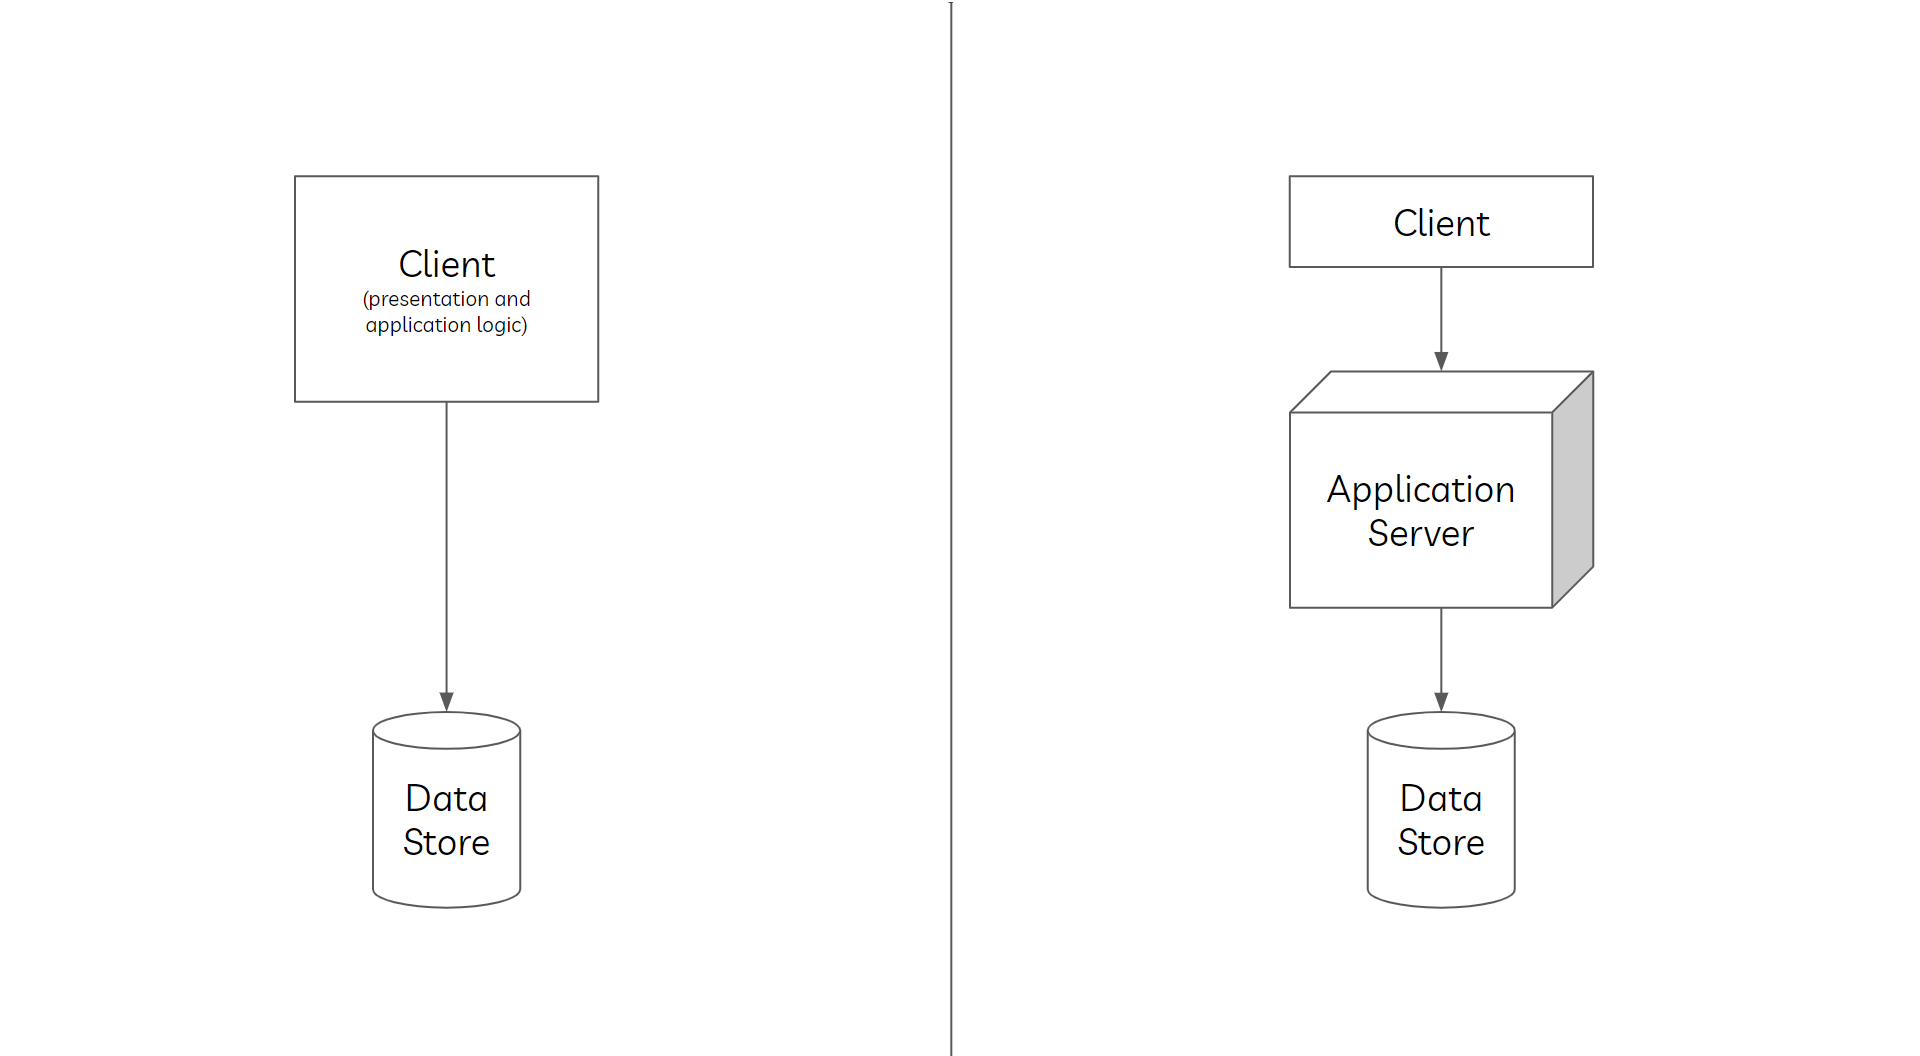
\includegraphics[width=\textwidth]{two-vs-three-tier-architecture.png}
    \caption[Two vs three tier architecture]{A diagram showing the difference
        between a two-tier \textit{(left)} and three-tier \textit{(right)}
        architecture. The two-tier architecture communicates to the data store
        without an intermediary application server, unlike the three-tier
        architecture.}
    \label{fig:two-vs-three-tier-architecture}
\end{figure}

With the introduction of this physical separation, the next challenge was the
structure of the software's code.  

Over an extensive period, applications built on top of the client-server model
extensively used the \textbf{\gls{mvc} pattern} \autocite{Pavlenko_etal_2020}.
Like the name suggests, this pattern describes 3 parts, that are used as
conceptual and architectural separations in the software. The business logic of
the application is encapsulated in the \textbf{model}, the presentation logic is
the responsibility of the \textbf{view}, and the \textbf{controllers} handle the
user actions in the views, and connect these actions to the appropriate models
and updated views.

However, according to \textcite{Leff_Raylfield_2001}, implementation of the
\gls{mvc} pattern for web applications in a client-server environment, brings up
the question of partitioning between servers and clients. Instinctively it is
clear that the views belong to the client and the models belong to the server,
but for the controllers, this separation is not so clear. Assigning the
controllers to the client-side would result in a \textit{fat client} again,
while assigning them to the server-side (the \textit{thin client} approach)
would often mean too many round-trips to the server must be performed on every
request. In practice, the workaround for this partitioning is a \textit{dual
\gls{mvc}} approach, which partitions the controllers between the client and the
server.


While the \gls{mvc} architecture pattern can give developers a cleaner
seperation of concerns in their code, it still produces a \textbf{tightly
coupled} solution. Any change would still mean the entire code would have to be
rebuilt and redeployed \autocite{Fowler_Microservices_2014}. This significantly
reduces development speed, as well as agility. \Glsplural{monolith} can also be considered
a  ``single point of failure'': whenever one part of the software is
malfunctioning, the whole system is crippled.


\subsection{The split-stack development model}
\label{ssec:split-stack}


In more recent times, developer teams started to adopt \textbf{split-stack
development}, where the \gls{gui} is handled in the so-called ``\gls{frontend}'' and
the business and data logic are dealt with by a ``\gls{backend}'' system. The
communication between these two parts can be carried out in multiple ways, but
one of the most common ways is via a (\gls{restful}) \gls{api}.

Decoupling the \gls{frontend} presentation logic from the \gls{backend} business logic
introduces some major benefits: \autocite{Dunkley_2016}
\begin{itemize}
    \item \textbf{Multiple clients}\\
    As it is not at all concerned with presentation logic, the same
    \gls{backend} service can now serve data to multiple different clients (e.g.
    web, desktop, mobile,...). To support a new type of client, only
    presentation logic has to be implemented.
    %
    \spacedItem  \textbf{Specialized teams}\\
    The split of \gls{frontend} and \gls{backend} allows developers to
    specialize themselves in these fields, yielding a deeper knowledge of the
    selected fields. 
    % 
    \spacedItem  \textbf{Independent technology stacks}\\
    Tying in with the previous point: as teams specialize, they desire and/or
    require more specialized technologies. The decoupling of front- and
    \gls{backend} removes any restraints on technology selection between the two
    areas. For example, \gls{frontend} developers can use client-side
    technologies and frameworks such as Typescript and React, while
    \gls{backend} developers can leverage server-side technologies such as .NET
    or Java. This also makes each individual solution more future-proof.
    %
    \spacedItem  \textbf{Simultaneous development}\\
    As a result of all outlined benefits above, and the basic concept of
    decoupling, teams can work independently, autonomously and therefore
    simultaneously. For example, a change to the visual styling of a website,
    will not require any of the server-side code to change, and will also not
    trigger a rebuild. 
    %
    \spacedItem  \textbf{Independent deployment and scaling}\\
    While a \gls{monolith} has to be deployed as one big program, teams can now
    deploy the \gls{frontend} and \gls{backend} solutions according to their
    needs. Often a static hosting solution is enough to publish a \gls{frontend}
    application, while a \gls{backend} service might need some serious
    infrastructure to remain operational.
\end{itemize}

Of course, these benefits also come at the cost of some drawbacks. 

Firstly, the fact that specialized teams can work on either the \gls{frontend}
and \gls{backend} separately and in their own technology stack is a double-edged
sword. While the benefits outlined above stay true; this also means that
developers are less flexible to switch teams in times of developer shortage or
approaching deadlines.

Secondly, the contract between the \gls{frontend} and \gls{backend} teams is a
well documented \gls{api} with clearly defined \glsplural{endpoint}. For \gls{restful}
web \gls{api} \textbf{documentation}, the OpenAPI
specification\hreffootnote{https://www.openapis.org/}, which is also known as
\textit{Swagger} documentation, provides a standardized way of defining this
contract \autocite{Koren_Klamma_2018}. Of course, time and effort needs to be
spent creating robust documentation. 

Thirdly, breaking changes have to be avoided at all times. \Gls{frontend} code
might depend on \gls{backend} \glsplural{endpoint} that will get deleted in an
upcoming update. This is not acceptable.
\textbf{Versioning}\hreffootnote{https://restfulapi.net/versioning/} provides a
way to keep supporting clients that rely on a version of the \gls{api} before
the breaking change was made.

Lastly, more relevant in the context of this thesis: while dividing the
\gls{frontend} from the \gls{backend} does provide benefits; in large, rapidly
scaling applications, it simply isn't enough. After a
\gls{frontend}-\gls{backend} split, one does still end up with a both a
\textbf{\gls{monolithic} \gls{backend}} and a \textbf{\gls{monolithic}
\gls{frontend}}. 

Shifting the frame of reference to the server-side: the \gls{backend}
\gls{monolith} still possesses the same downsides the overall \gls{monolith} had
introduced: one change in the logic and the entire application has to be
rebuilt and redeployed. Also, the issue of scaling still persists: the server
can be updated with more powerful hardware (vertical scaling) or the \textit{entire}
server-side application can be replicated on different servers, with a
\gls{load-balancer} deciding how to distribute incoming requests (horizontal scaling).
Keyword here is \textit{``entire''}, as no specific part of the server-side
application can be scaled up independently. 


\subsection{Microservices} 
\label{ssec:microservices}

Due to an increased business interest in software services, the focus for
choosing a software architectural style and paradigm shifted towards reusability
and robustness. According to \textcite{Dragoni_etal_2018}, This was
characterized by the shift to more modular, loosely coupled applications. The
benefits of which were outlined in the previous section. The \gls{soa} pattern
emerged as a step in this direction. Initially, the goal was to devise software
services as a way to interface with larger software systems (which were often
monolithic) via messages, using common messaging protocols (e.g. \gls{http},
\gls{soap} or \gls{xml}).

Taking this approach further, by not necessarily integrating with existing
\gls{monolithic} applications, but using the service-oriented approach to design,
develop and deploy self-contained and autonomous software services, is what the
\gls{ma} is about.\footnote{While conceptually derived from \gls{soa}, labeling
the \gls{ma} as an implementation of \gls{soa} is highly debated. Read more on
\hrefself{https://martinfowler.com/articles/microservices\#MicroservicesAndSoa}.}


A visual overview of the \gls{ma} is shown in Figure~\ref{fig:microservices}.


\begin{figure}
    \centering
    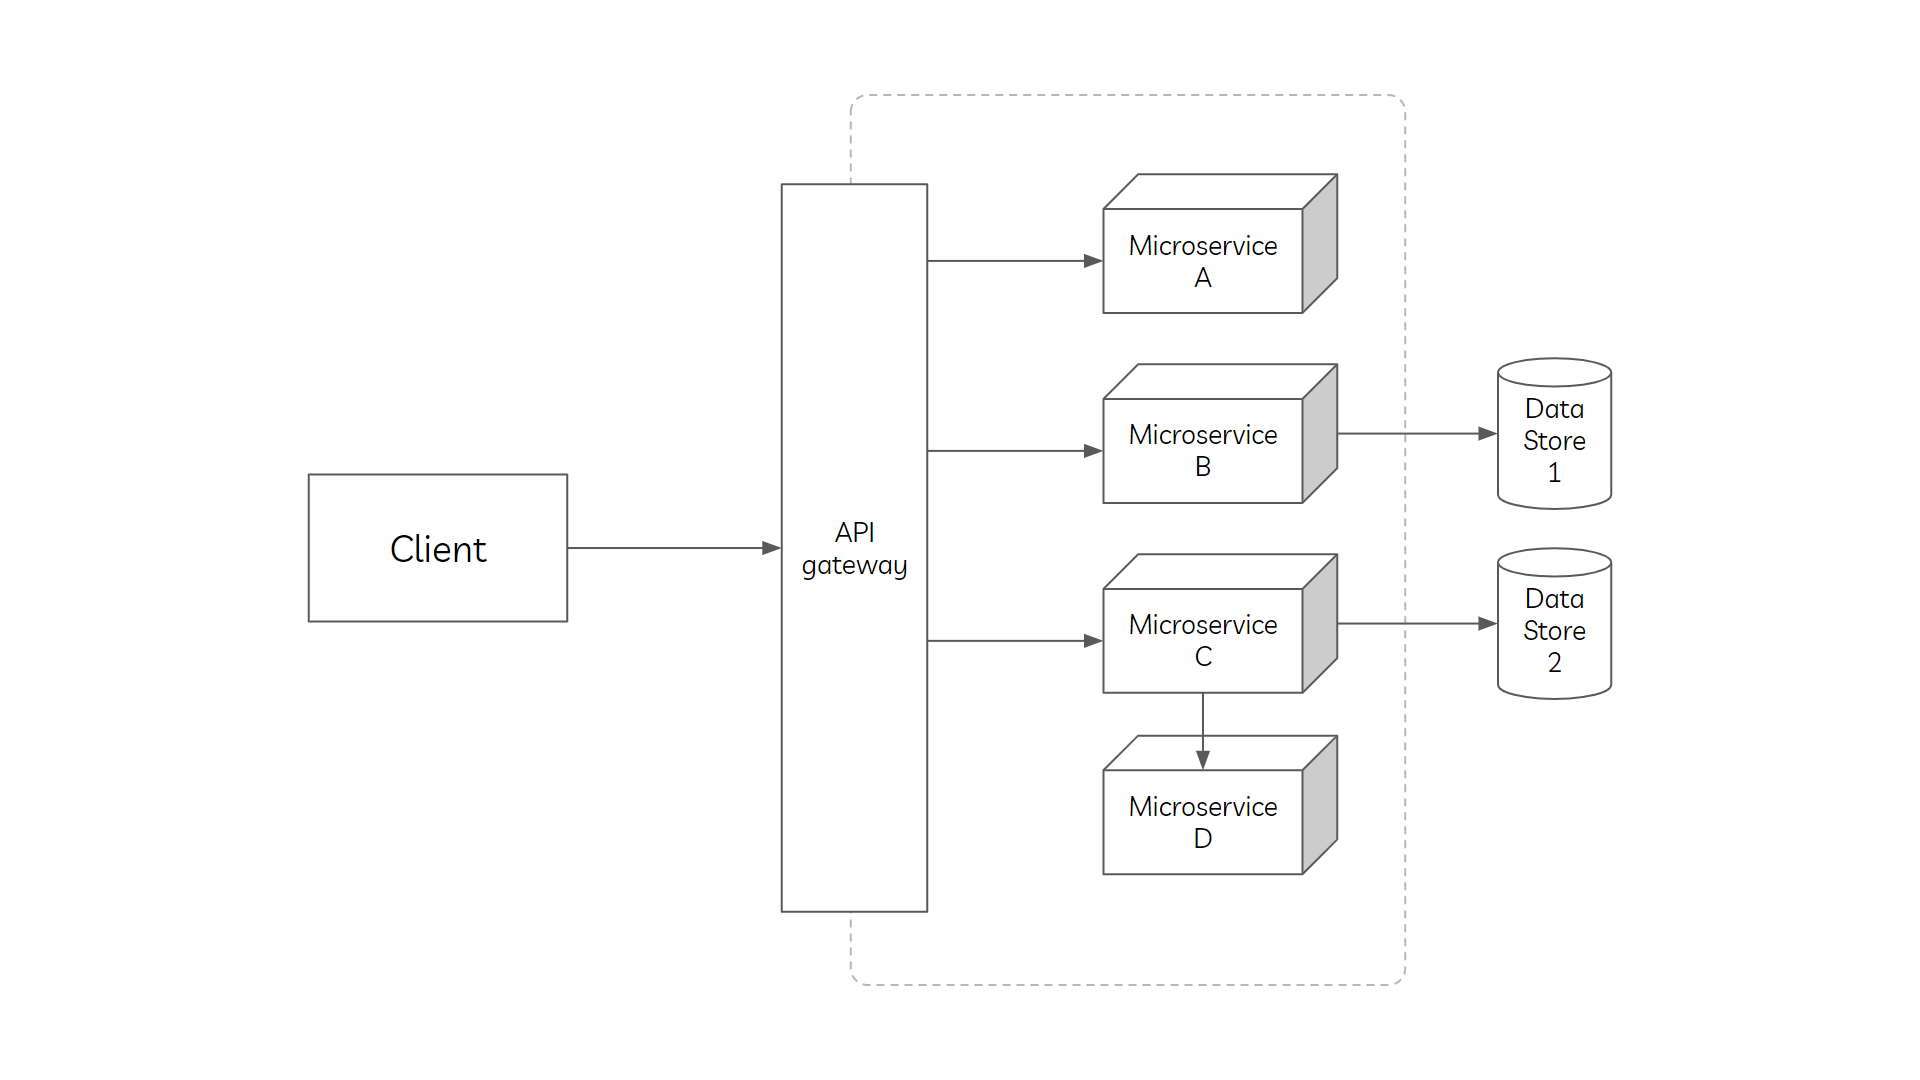
\includegraphics[width=\textwidth]{microservices.png}
    \caption[Microservices]{A diagram showing an example of a \gls{ma} with
    services A through D.}
    \label{fig:microservices}
\end{figure}


\subsubsection{Principles of the microservice architecture}
\label{principles-of-the-mfa}

The \gls{ma} is built on a few basic principles \autocite{Dragoni_etal_2018}
\autocite{Dragoni_etal_2017} \autocite{Fowler_Microservices_2014}
\autocite{Gysels_2020} \autocite{Newman_2015}:

\begin{itemize}
    \item \textbf{Small codebases managed by small teams}\\
    Codebases are generally smaller in size, at least small enough to be managed
    by a small team (this typically means less than 10 people).
    % 
    \spacedItem \textbf{Focused on a specific business need}\\
    Every \gls{microservice} should be centered around a specific business need
    or domain, so that the responsibility of every \gls{microservice} is clearly
    defined\footnote{This can be seen as the application of the Single
    Responsibility Principle to independent services}, and there is an alignment
    between the business capabilities and the software architecture. 
    %
    \spacedItem \textbf{Modular, decoupled and independent}\\
    According to \textcite{Evans_2004}, using a software model in a well defined
    \textit{bounded context}, without worrying about the applicability of the
    model to other contexts, is key to keeping the context \textit{pure} and
    avoiding confusion.\\
    Every \gls{microservice} should be built, tested and deployed
    individually and in isolation. 
    %
\end{itemize}

The only form of \textbf{communication} between individual
\glsplural{microservice} is a uniform communication mechanism via network calls.
In practice, the most commonly used mechanisms are the request-response
mechanism using for example \gls{http} (with \gls{rest} or \gls{rpc}) or the
event-based mechanism using an \textit{event bus}\footnote{e.g. Apache
Kafka, RabbitMQ, Azure Service Bus, ...}. The latter mechanism is generally
encouraged as event-based collaboration is highly decoupled
\autocite{Newman_2015}.

Communication with the ``outside world'' (i.e. with a client) is usually done
using a facade over all the underlying \glsplural{microservice}: usually called
an \textit{\gls{api_gateway}}. This service can aggregate content gathered from
multiple \gls{backend} calls, and serve it. Whenever this layer becomes too large, or
becomes bloated with logic, a \textit{\gls{bff}} pattern can be more useful:
this is essentially equivalent to an \textit{\gls{api_gateway}} per client. This
is shown in Figure~\ref{fig:bff}.


\begin{figure}
    \centering
    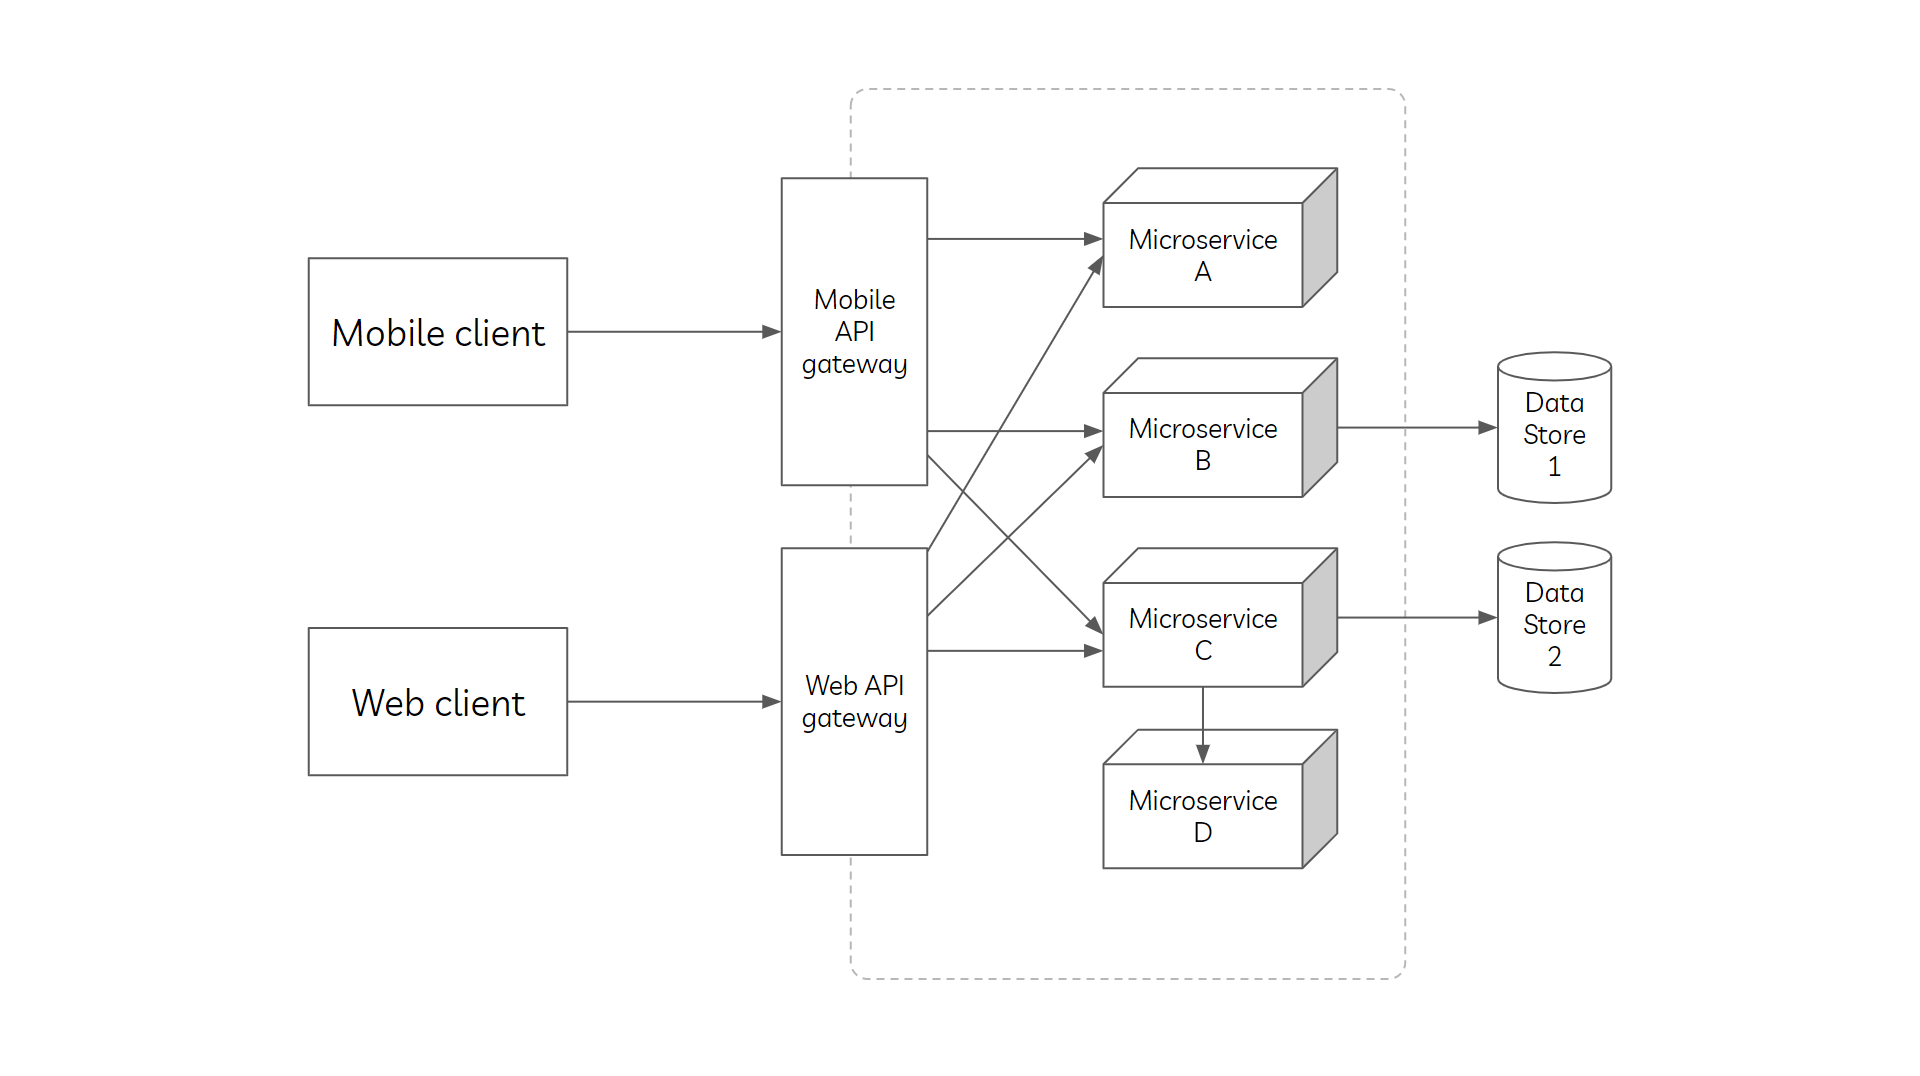
\includegraphics[width=\textwidth]{bff.png}
    \caption[Backend for frontend pattern]{A diagram showing an example of the
    \gls{bff} pattern with a mobile and a web client.}
    \label{fig:bff}
\end{figure}


As for \textbf{authentication}, according to \textcite{Newman_2015}, a \gls{sso}
solution is often used, whereby the user can authenticate with an
\textit{identity provider}.


\subsubsection{Benefits of using a microservice architecture}

Below some of the major benefits of the \gls{ma} are outlined:

\begin{itemize}
    \item \textbf{Technology independence}\\
    Explanation of this benefit can be directly borrowed from
    \fullref{ssec:split-stack}. Choosing the right technologies for the problem
    is obviously very beneficial. \textit{Not every problem is a nail, and not
    every solution is a hammer} \autocite{Fowler_Microservices_2014}. 
    %
    \spacedItem \textbf{Scalibility and elasticity}\\
    Scaling a \gls{ma} does not require reduplication of the entire software
    system. Every component can be scaled as needed with respect to their
    expected or measured load. Microservices are often deployed using
    \textit{containers} using technologies such as
    Docker\hreffootnote{https://docker.com}, which can be managed in
    \textit{clusters} by other technologies such as
    Kubernetes\hreffootnote{https://kubernetes.io}. This way, scaling can be
    done \textit{elastically}: dynamically according to the load.
    \autocite{Dragoni_etal_2018}
    %
    \spacedItem \textbf{Availibility and resilience to failure}\\
    While the methods used for scaling can improve performance and make it
    possible to cope with a high load on a software system, the same methods can
    also be applied to create redundancy and therefore resilience to failure.
    Also, because a defect in one \gls{microservice} does not lead to the
    crashing or malfunctioning of the entire system. When errors do come
    forward, they are easier to locate in the narrow scope of the
    \gls{microservice}. Additionally, when upgrading a microservice,
    instances of the old and new versions can run side by side, aiding in a
    smooth transition between them, and less or no downtime.
    \autocite{Dragoni_etal_2017}
    %
    \spacedItem \textbf{Better teams}\\
    The term ``better'' here is used in place of many different adjectives.
    Because of the limited scope a \gls{microservice} has, teams gain a deeper
    understanding of the business domain, and feel a greater sense of ownership
    over the features they develop. Combining this with the smaller codebases
    and shorter release cycles, teams tend to get smaller and more productive
    \autocite{Newman_2015}.
    %
\end{itemize}

\subsubsection{Challenges and limitations of the microservice architecture}
\label{sssec:microservice-challenges}

While lots of the benefits of the \gls{ma} aid in enabling distributed
development, the architecture cannot be regarded as a \textit{silver bullet}. In
what follows, some of the challenges of the \gls{ma} are outlined, based in part
on a literature review by \textcite{Soldani_2018}. Depending on the perspective
of the reader, some of these can also be considered to be drawbacks.

\textbf{Partitioning the services} tends to be a big challenge in the design
phase of \gls{microservice} development. It is often difficult to slice up the
business capabilities into well-defined categories. Another challenge in the
conceptual phase is establishing a clear strategy for \textbf{communication}
mechanisms: \gls{microservice} intercommunication should have clear contracts to
ensure their compatibility.

During the development phase, because of the distributed nature of the \gls{ma},
issues concerning data come up frequently. To ensure the necessary decoupling,
each \gls{microservice} should have a dedicated data store or database. If there is
data duplication, this can raise issues with \textbf{data consistency}.
Operating with distributed data stores also brings up the issue of
\textbf{distributed transactions}: if one of the services fails to perform a
database operation, what will happen to the principle of a transaction?

Another challenge in the development phase is designing and writing adequate
\textbf{tests}. Because of their independent nature, unit tests are easier or in
the worst case simply unaffected by the \gls{ma}. Performance testing, integration
testing and end-to-end testing, however, become more difficult because the
system has to be tested from the outside. Often multiple services have to be
spun up to be able to do a test properly, increasing the performance cost of the
tests, and lowering their reliability.\footnote{See also
\hrefself{https://blog.indrek.io/articles/challenges-of-testing-microservices/}}

If the \gls{microservice}-application is running, most of the challenges
of the \gls{ma} boil down to \textbf{increased operational complexity}:
debugging, logging, monitoring, service coordination, etc. 

It is also worth noting that the \gls{ma} requires a certain \textbf{developer
skill and knowledge}, that might not be readily available in a company or
organization.
